\FloatBarrier
\section{Controls, ablations, and two-sided baselines}
\label{sec:controls_ablations}

Because \mname{MuonT} already removes forward input ill-conditioning, the incremental output-side improvement is a few millinats—a scale where numerical execution differences, short-horizon hyperparameter tuning, or altered regularization can confound optimizer comparisons. We pair execution-path and learning-rate controls with targeted factor-placement ablations and long-horizon comparisons against recent two-sided polar optimizers.

\subsection{Execution-path and learning-rate controls}
\label{sec:falsification}

\mname{Null-WT} executes synchronous cotangent capture, cross-rank pooling, and inverse-root construction identically to the two-sided pipeline, then substitutes identity output factors ($L=\hat L=I$) at the update. While it does not separately test asynchronous scheduling, it directly tests whether altered kernel batching and mixed-precision accumulation manufacture an apparent gain. At $\eta=0.02263$ on 130M seed 0, \mname{Null-WT} finishes just $0.0003$ nats below \mname{MuonT}, compared with $0.0043$ nats for \mname{WT-MLP-Lag} (\Cref{fig:confounds}(b,c), \Cref{tab:controls}), making execution-path drift an unlikely explanation for the improvement.

\begin{figure}[t]
 \centering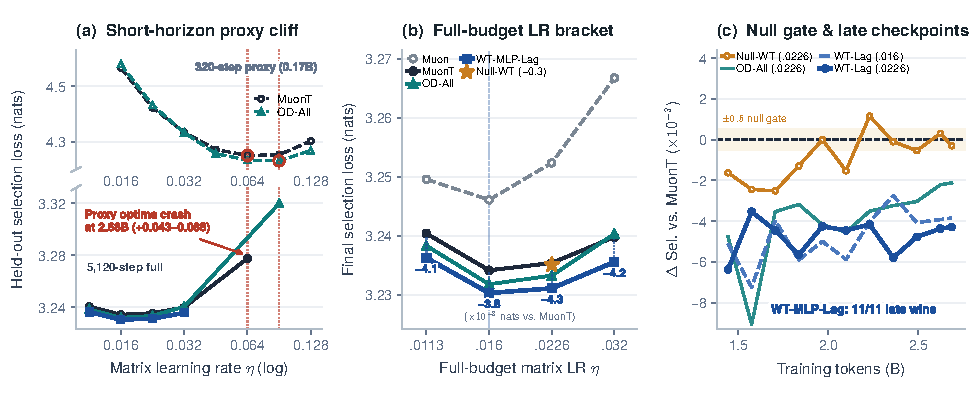
\includegraphics[width=\textwidth]{fig4_confounds_lr_null.pdf}
 \caption{\textbf{The output-side gain survives full-budget learning-rate bracketing and a matched execution-path control.}
 \textbf{(a)} Matrix learning rates chosen on a compressed 320-step proxy sweep transfer poorly to the full 5,120-step budget.
 \textbf{(b)} Full-budget held-out loss across $\eta\in\{0.0113,0.0160,0.0226,0.0320\}$, alongside the matched-path identity control (\mname{Null-WT}).
 \textbf{(c)} Second-half trajectory differences from \mname{MuonT} at $\eta=0.02263$: \mname{Null-WT} stays near zero while \mname{WT-MLP-Lag} wins all 11 late checkpoints. All panels use 130M, seed 0 (2.68B tokens).}
 \label{fig:confounds}
\end{figure}

\begin{table}[tbp]\centering\small
\setlength{\tabcolsep}{5.2pt}
\caption{\textbf{Seed-0 learning-rate bracket, execution-path control, and short-schedule transfer at 130M (2.68B tokens).} Entries are final held-out losses in nats across the complete four-point bracket (bold marks each row's full-budget minimum, $\eta^*=0.0160$ for every method); $\Delta_{0.0226}$ is the paired difference from Muon at $\eta=0.02263$ in millinats where Null-Ctrl is evaluated. The rightmost column transfers each checked arm's 320-step argmax learning rate (\Cref{tab:lr_cliff}) to the full 5,120-step schedule.}\label{tab:controls}
\begin{tabularx}{\textwidth}{@{}>{\raggedright\arraybackslash}Xrrrrrr@{}}
\toprule
& \multicolumn{4}{c}{Full-budget held-out loss $\Lsel$ (nats)} & & \\
\cmidrule(lr){2-5}
Method & $0.0113$ & $0.0160$ & $0.0226$ & $0.0320$ & $\Delta_{0.0226}$ (mnats) & 320-step $\eta^* \to$ full \\
\midrule
Muon & 3.2496 & \textbf{3.2461} & 3.2524 & 3.2667 & $+0.00$ & --- \\
MuonT & 3.2404 & \textbf{3.2342} & 3.2354 & 3.2398 & $-16.96$ & $0.0640 \to 3.2775$ \\
Null-Ctrl & --- & --- & 3.2351 & --- & $-17.26$ & --- \\
Muon2-Diag & 3.2383 & \textbf{3.2318} & 3.2333 & 3.2403 & $-19.08$ & $0.0905 \to 3.3200$ \\
\rowcolor{rowtint}[0pt][0pt]\textbf{Muon2-ExpDiag} & 3.2363 & \textbf{3.2303} & 3.2311 & 3.2356 & $\mathbf{-21.25}$ & --- \\
\bottomrule\end{tabularx}
\end{table}


Short-schedule learning-rate screening is a second major pitfall~\citep{choi2019empirical,schmidt2021crowded,kaddour2023nodata,dang2026batchsize}. A 320-step proxy sweep selects $\eta\in[0.064,0.0905]$—roughly four times the full-budget optimum—and transferring those rates to 5,120 steps degrades final loss by $0.04\text{--}0.09$ nats, swamping second-side differences (\Cref{fig:confounds}(a), \Cref{tab:controls}; complete sweep in \Cref{app:appendix_lr,tab:lr_cliff}). Across the full 2.68B-token bracket $\eta\in\{0.01131,0.016,0.02263,0.032\}$, all four core methods share a strict interior minimum at $\eta^*=0.0160$, and \mname{WT-MLP-Lag} outperforms \mname{MuonT} by $0.0038\text{--}0.0043$ nats at every matched rate.

\subsection{Factor placement, exponent split, and one-step lag}
\label{sec:ablations}

\Cref{tab:ablations} and \Cref{fig:ablations_related}(a) isolate each design element of \mname{WT-MLP-Lag} at 130M (complete 19-arm multi-wave ledger in \Cref{app:ablations,tab:ablations_full}):
\begin{itemize}
 \item \textbf{Dense input whitening remains indispensable.} Replacing input factors with dense output factors alone (\mname{Abl-OutOnly}, $+8.71$ mnats; which also switches weight decay to $\hat L^2 W$) or diagonalizing both sides (\mname{Abl-BothDiag}, $+18.01$ mnats) performs substantially worse than \mname{MuonT}. Diagonalizing the $\dff$-wide \texttt{down} input alongside expanded outputs (\mname{WT-Sym-Lag}, $-1.13$ mnats) likewise sacrifices most of \mname{WT-MLP-Lag}'s gain ($-5.68$ mnats), confirming the input--output asymmetry identified in \Cref{sec:dichotomy}.
 \item \textbf{Both output width classes and both $(-1/2,-1/8)$ factors contribute.} Dropping preconditioning on \texttt{gate,up} (\mname{Abl-No2048}, $-3.07$ mnats) loses roughly half of synchronous \mname{WT-MLP}'s gain ($-6.58$ mnats), whereas upgrading \texttt{gate,up} from diagonal to dense spectral factors (\mname{DT-All}, $-5.78$ mnats) yields no held-out benefit despite raising median step-time overhead to $+21.6\%$. Applying only the post-polar outer factor (\mname{Abl-OuterDense}, $-3.98$ mnats) also underperforms the inner/outer pair.
 \item \textbf{One-step lag retains quality while halving exposed overhead.} Comparing synchronous \mname{WT-MLP} ($-6.58$ mnats) with lagged \mname{WT-MLP-Lag} ($-5.68$ mnats), and synchronous \mname{DT-All} ($-5.78$ mnats) with \mname{DT-All-Lag} ($-5.89$ mnats), retains nearly all of the held-out improvement while cutting unified 8-GPU median step time from $1.221$ to $1.155$\,s ($+11.3\%$ to $+5.3\%$). Because these exploratory arms span implementation waves, they provide provisional component evidence that the fresh-seed campaign in \Cref{sec:scaling} confirms end-to-end.
\end{itemize}

\begin{table}[!htb]\centering\small
\setlength{\tabcolsep}{4.4pt}
\caption{\textbf{Factor-placement, exponent, and scheduling ablations at 130M (seed 0, 2.68B tokens).} Inputs and outputs list the $(\dm / \dff)$ operator assignment under the $(-1/2,-1/8)$ split unless noted; Muon uses $\eta^*=0.016$ and all other arms use $\eta=0.02263$. Loss columns report cohort-adjusted 11-checkpoint second-half mean differences (millinats) relative to Muon (negative favors the row method; MuonT sits at $-5.50$ and $-5.34$ mnats). Step $\Delta t$ is median step-time overhead relative to Muon in the unified 8-GPU benchmark (\Cref{tab:bench19}), matching \Cref{fig:mech_pareto}(b,c). All 19 exploratory arms appear in \Cref{tab:ablations_full}.}\label{tab:ablations}
\begin{tabularx}{\textwidth}{@{}>{\raggedright\arraybackslash}Xllcrrr@{}}
\toprule
Method & Inputs ($\dm / \dff$) & Outputs ($\dm / \dff$) & Lag & Late $\Delta\Lsel$ & Late $\Delta\Lc$ & Step $\Delta t$ \\
\midrule
\addlinespace[2pt]\multicolumn{7}{@{}l}{\textit{Reference baselines and execution-path control}}\\
Muon & $I$ / $I$ & $I$ / $I$ & --- & $+0.00$ & $+0.00$ & $+0.0\%$ \\
MuonT & Dense / Dense & $I$ / $I$ & --- & $-5.50$ & $-5.34$ & $+1.5\%$ \\
Null-Ctrl & Dense / Dense & $I$ / $I$ (solved) & 0 & $-6.15$ & $-7.39$ & $+13.9\%$ \\
\addlinespace[4pt]\multicolumn{7}{@{}l}{\textit{Replacing or weakening input whitening}}\\
Abl-BothDiag & Diag / Diag & Diag / Diag & 0 & $+12.51$ & $+12.34$ & $+1.1\%$ \\
Abl-OutOnly & $I$ / $I$ & Dense / Dense & 0 & $+3.20$ & $+5.55$ & $+31.7\%$ \\
Abl-SymDiag & Dense / Diag & Dense / Diag & 1 & $-6.63$ & $-6.95$ & $+4.8\%$ \\
\addlinespace[4pt]\multicolumn{7}{@{}l}{\textit{Output projection role and inner/outer exponent placement}}\\
Abl-NoExp & Dense / Dense & Dense / $I$ & 0 & $-8.57$ & $-7.97$ & $+13.7\%$ \\
Abl-OuterDense & Dense / Dense & $\hat L$ Dense ($L=I$) & 0 & $-9.48$ & $-10.12$ & $+28.2\%$ \\
Muon2-Diag & Dense / Dense & Diag / Diag & 0 & $-10.01$ & $-8.95$ & $+3.7\%$ \\
\addlinespace[4pt]\multicolumn{7}{@{}l}{\textit{Dense two-sided ceiling versus expansion-diagonal outputs and one-step lag}}\\
Muon2-Dense & Dense / Dense & Dense / Dense & 0 & $-11.29$ & $-11.72$ & $+23.3\%$ \\
Muon2-Dense (lag) & Dense / Dense & Dense / Dense & 1 & $-11.40$ & $-11.21$ & $+18.2\%$ \\
Muon2-ExpDiag (sync) & Dense / Dense & Dense / Diag & 0 & $\mathbf{-12.09}$ & $-11.42$ & $+12.9\%$ \\
\rowcolor{rowtint}[0pt][0pt]\textbf{Muon2-ExpDiag} & Dense / Dense & Dense / Diag & 1 & $\mathbf{-11.19}$ & $\mathbf{-10.33}$ & $+6.8\%$ \\
\bottomrule\end{tabularx}
\end{table}


\begin{figure}[t]
 \centering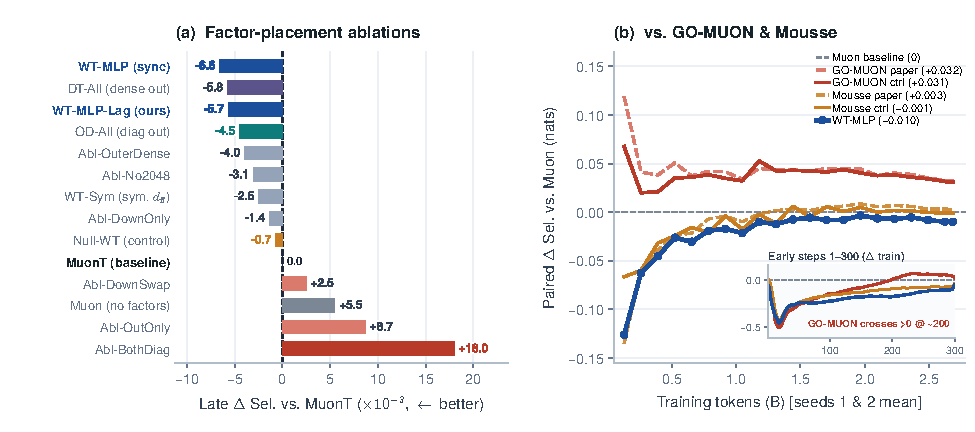
\includegraphics[width=\textwidth]{fig7_ablations_and_related.pdf}
 \caption{\textbf{Width-thresholded output preconditioning outperforms factor-placement ablations and alternative two-sided polar baselines.}
 \textbf{(a)} Second-half held-out loss differences from cohort \mname{MuonT} across 14 configurations at 130M, 2.68B tokens (seed 0; exploratory multi-wave settings in \Cref{tab:ablations,tab:ablations_full}).
 \textbf{(b)} Held-out trajectories relative to \mname{Muon} under shared isotropic matrix decay ($\lambda=0.1,\eta=0.032$, mean of fresh seeds 1 and 2). Inset: early training loss over steps 1--300, where \mname{GO-MUON}'s initial lead reverses near step 200 while \mname{WT-MLP} retains its advantage through 2.68B tokens.}
 \label{fig:ablations_related}
\end{figure}

\subsection{Comparison with two-sided polar baselines}
\label{sec:related_baselines}

We also compare synchronous \mname{WT-MLP} against two recent methods that combine second-order statistics with polar updates: \mname{GO-MUON}~\citep{che2026gomuon}, which applies symmetric $(-1/4,-1/4)$ activation/cotangent powers with norm grafting, and \mname{Mousse}~\citep{zhang2026mousse}, which applies symmetric $(-1/8,-1/8)$ powers of full gradient Gram matrices $GG^{\Tr}$ and $G^{\Tr}G$ with norm grafting. For each baseline, we evaluate both a controlled profile sharing our EMA, damping, refresh cadence, and $\Nten$ map, and a paper profile following method-specific choices, under shared isotropic matrix decay ($\lambda=0.1,\eta=0.032$) across two fresh seeds (\Cref{tab:related}, \Cref{fig:ablations_related}(b); a controlled recipe comparison rather than independent hyperparameter tuning).

\begin{table}[!htb]\centering\small
\setlength{\tabcolsep}{4.2pt}
\caption{\textbf{Two-sided polar baselines under a shared isotropic-decay recipe (130M, 2.68B tokens).} Entries average fresh seeds 1 and 2 at $\eta=0.032$ and $\lambda=0.1$ on the standalone synchronous harness. Held-out is final $\Lsel$ in nats; $\Delta$ columns are millinats from Muon (Late-11 averages the second-half checkpoints); Step is median seconds per update.}\label{tab:related}
\begin{tabularx}{\textwidth}{@{}ll>{\raggedright\arraybackslash}Xrrrrr@{}}
\toprule
Method & Profile & Moments \& Exponents & Held-out & $\Delta\Lsel$ & Late-11 $\Delta$ & $\Delta\Lc$ & Step (s) \\
\midrule
Muon & Reference & None; $\Nten(U)$ & 3.2074 & $+0.00$ & $+0.00$ & $+0.00$ & 1.15 \\
Mousse & Paper & $GG^{\Tr}, G^{\Tr}G$; $(-1/8,-1/8)$ + graft & 3.2102 & $+2.78$ & $+4.85$ & $+3.25$ & 1.13 \\
Mousse & Controlled & $GG^{\Tr}, G^{\Tr}G$; $(-1/8,-1/8)$ + graft & 3.2064 & $-0.98$ & $+1.23$ & $-1.92$ & 1.20 \\
GO-MUON & Controlled & $C, B$; $(-1/4,-1/4)$ + graft & 3.2384 & $+30.98$ & $+38.22$ & $+29.36$ & 1.59 \\
GO-MUON & Paper & OAS $C, B$; SVD + graft & 3.2395 & $+32.08$ & $+39.71$ & $+30.48$ & 2.02 \\
\rowcolor{rowtint}[0pt][0pt]\textbf{Muon2-ExpDiag} & Sync ($\tau=0$) & $C, B$ (\texttt{gate,up} diag); $(-1/2,-1/8)$ & \textbf{3.1975} & $\mathbf{-9.90}$ & $\mathbf{-7.14}$ & $\mathbf{-9.91}$ & 1.36 \\
\bottomrule\end{tabularx}
\end{table}


At 2.68B tokens, both \mname{GO-MUON} profiles finish roughly $0.03$ nats worse than \mname{Muon}—reversing an early 200-step training-loss lead—while both \mname{Mousse} profiles finish close to \mname{Muon}. Under the same isotropic decay, \mname{WT-MLP} lowers held-out loss by $0.0099$ nats below \mname{Muon}, showing that its benefit does not depend on \mname{MuonT}'s shaped weight decay. Two operator differences are consistent with this gap: a gradient Gram $GG^{\Tr}=\sum_{i,j}\langle x_i,x_j\rangle\delta_i\delta_j^{\Tr}$ entangles cotangents with activation inner products and cross-token terms that separate $(C,B)$ moments avoid, and steeper $(-1/4,-1/4)$ outer inverse powers with norm grafting place heavier weight on noisy low-variance cotangent modes—though because these baselines change multiple choices together, this comparison does not isolate a single causal factor.
